\documentclass{report} % article, book
\usepackage{array}
\usepackage{graphicx}
\usepackage[table,xcdraw]{xcolor}
\usepackage{appendix}
\usepackage{bookmark}
\usepackage{hyperref}
\hypersetup{ % Setting the reference colors
    colorlinks,
    linkcolor={red!10!black},
    citecolor={blue!50!black},
    urlcolor={blue!80!black}
}
\usepackage[english]{babel}
\usepackage{csquotes}
\usepackage{linebreaker}
\usepackage{enumitem}
\setlist[itemize]{leftmargin=*, itemsep=0.2em}
\setlist[enumerate]{leftmargin=*}
\usepackage{multicol} % For making 2 columns 
\setlength{\columnsep}{20pt} % Column separation
\setlength{\columnseprule}{0.5pt} % Column separation rule thickness
\usepackage[parfill]{parskip}
\usepackage{listings} % For writing code lines
\usepackage{fontspec}
\setmainfont{Times New Roman}
\usepackage{geometry}
 \geometry{ % APA all lines need to be equal 24mm
 a4paper,
 left=24mm,
 top=24mm,
 right=24mm,
 bottom=24mm,
}
\usepackage[toc,acronym]{glossaries} % Glossary package, with acronym and ToC support
\usepackage[% APA Citation 7th Edition
backend=biber,
natbib=true,
style=apa,
]{biblatex}
\addbibresource{references.bib}
\makeglossaries
\definecolor{darkblue}{rgb}{0.0, 0.0, 0.55}
\definecolor{codeGreen}{rgb}{0,0.6,0}
\definecolor{codeGray}{rgb}{0.5,0.5,0.5}
\definecolor{backcolour}{rgb}{0.95,0.95,0.92}

\lstdefinelanguage{JavaScript}{ % Define JavaScript language in listing
  keywords={break, case, catch, continue, debugger, default, delete, do, else, false, finally, for, function, if, 
    in, instanceof, new, null, return, switch, this, throw, true, try, typeof, var, void, while, with, const,},
  keywordstyle=\color{blue}\bfseries,
  ndkeywordstyle=\color{darkgray}\bfseries,
  identifierstyle=\color{black},
  sensitive=false,
  comment=[l]{//},
  morecomment=[l]{//},
  morecomment=[s]{/*}{*/},
  commentstyle=\color{purple}\ttfamily,
  stringstyle=\color{red}\ttfamily,
  morestring=[b]',
  morestring=[b]",
  ndkeywords={class, export, boolean, throw, implements, import, this, constructor, boolean, string, number},
  keywordstyle=\color{blue}\bfseries,
  stringstyle=\color{red}\ttfamily,
  sensitive=true
}

\lstdefinelanguage{XML} { % Define XML language in listing
    morestring=[b]",
    morestring=[s]{>}{<},
    morecomment=[s]{<?}{?>},
    stringstyle=\color{black},
    identifierstyle=\color{darkblue},
    keywordstyle=\color{cyan},
    morekeywords={xmlns,version,type}
}

\lstdefinelanguage{JSON} { % Define JSON language in listing
    morestring=[b]",
    morestring=[d]',
    basicstyle=\normalfont\ttfamily,
    commentstyle=\color{eclipseStrings},
    stringstyle=\color{eclipseKeywords},
    numbers=left,
    numberstyle=\scriptsize,
    stepnumber=1,
    numbersep=8pt,
    showstringspaces=false,
    breaklines=true,
    frame=lines,
    backgroundcolor=\color{gray},
    string=[s]{"}{"},
    comment=[l]{:"},
    literate=
     *{0}{{{\color{numb}0}}}{1}
      {1}{{{\color{numb}1}}}{1}
      {2}{{{\color{numb}2}}}{1}
      {3}{{{\color{numb}3}}}{1}
      {4}{{{\color{numb}4}}}{1}
      {5}{{{\color{numb}5}}}{1}
      {6}{{{\color{numb}6}}}{1}
      {7}{{{\color{numb}7}}}{1}
      {8}{{{\color{numb}8}}}{1}
      {9}{{{\color{numb}9}}}{1}
      {:}{{{\color{punct}{:}}}}{1}
      {,}{{{\color{punct}{,}}}}{1}
      {\{}{{{\color{delim}{\{}}}}{1}
      {\}}{{{\color{delim}{\}}}}}{1}
      {[}{{{\color{delim}{[}}}}{1}
      {]}{{{\color{delim}{]}}}}{1},
}

\lstset{% Listing settings
    backgroundcolor=\color{lightgray},
    extendedchars=true,
    basicstyle=\footnotesize\ttfamily,
    showstringspaces=false,
    showspaces=false,
    numbers=left,
    numberstyle=\footnotesize,
    numbersep=9pt,
    tabsize=2,
    breaklines=true,
    showtabs=false,
    columns=fullflexible,
    commentstyle=\color{gray}\upshape,
    breakatwhitespace=true,
    morekeywords={encoding,
        xs:schema,xs:element,xs:complexType,xs:sequence,xs:attribute}
    captionpos=b,
}

\newglossaryentry{Pentest}
{
    name=\acrshort{pentest},
    description={\acrshort{aka} ethical hacking, is a simulated cyberattack where professional ethical hackers break into corporate 
    networks to find weaknesses (\cite{pentest})
    }  
}
\newglossaryentry{CRM}
{
    name=\acrshort{crm},
    description={is a technology for managing all your company's relationships and interactions with 
    customers and potential customers. It provides a centralized \acrshort{db} or system for storing and organizing customer 
    data, as well as tools for managing sales, marketing, customer service, and other aspects of customer relationships. 
    A \acrshort{crm} system helps companies stay connected to customers, streamline processes, and improve profitability (\cite{crm})
    }
}
\newglossaryentry{RMM} {
    name=\acrshort{rmm},
    description={is a software platfomr that helps \acrshort{msp}s remotely monitor and manage their clients' endpoints, networks, 
    and computers (\cite{rmm}).}
}
\newglossaryentry{API} {
    name=\acrshort{api},
    description={is a software intermediary that allows two applications to talk to each other (\cite{api}). In other words, an 
    \acrshort{api} is the messenger that delivers request to the provider that was requested from and then delivers the response 
    back. (\cite{api})
    }
}
\newglossaryentry{AD} {
    name=\acrshort{ad},
    description={is a directory service developed by Microsoft for Windows domain network. It provides a database and set of 
    services that connect users with the network resources they need to get their work done(\cite{api})
    }
}

\newacronym{2fa}{2FA}{Two-Factor Authentication}
\newacronym{ad}{AD}{Active Directory}
\newacronym{ai}{AI}{Artificial Intelligence}
\newacronym{aka}{A.K.A.}{Also Known As}
\newacronym{apa}{APA}{American Psychological Association}
\newacronym{api}{API}{Application Programming Interface}
\newacronym{apt}{APT}{Advanced Persistent Threat}
\newacronym{att&ck}{ATT\&CK}{Adversarial Tactics, Techniques, and Common Knowledge}
\newacronym{av}{AV}{Anti-Virus}
\newacronym{baas}{BaaS}{Back-end as a Service}
\newacronym{bv}{B.V.}{Besloten Vennootschap}
\newacronym{c&c}{C&C}{Command-and-Control}
\newacronym{cmd}{CMD}{Command Prompt}
\newacronym{cfo}{CFO}{Chief Financial Officer}
\newacronym{cso}{CSO}{Chief Security Officer}
\newacronym{ciso}{CISO}{Chief Information Security Officer}
\newacronym{cdo}{CDO}{Chief Data Officer}
\newacronym{cco}{CCO}{Chief Communications Officer}
\newacronym{ceo}{CEO}{Chief Executive Officer}
\newacronym{coo}{COO}{Chief Operating Officer}
\newacronym{cto}{CTO}{Chief Technology Officer}
\newacronym{cmo}{CMO}{Chief Marketing Officer}
\newacronym{cio}{CIO}{Chief Information Officer}
\newacronym{clo}{CLO}{Chief Legal Officer}
\newacronym{cbdo}{CBDO}{Chief Business Development Officer}
\newacronym{cro}{CRO}{Chief Risk Officer}
\newacronym{cae}{CAE}{Chief Audit Executive}
\newacronym{cd}{CD}{Continuous Delivery/Deployment}
\newacronym{chro}{CHRO}{Chief Human Resources Officer}
\newacronym{ci}{CI}{Continuous Integration}
\newacronym{csv}{CSV}{Comma-Separated Values}
\newacronym{crm}{CRM}{Customer Relationship Management}
\newacronym{csp}{CSP}{Cloud Service Provider}
\newacronym{ct}{CT}{Creative Technology}
\newacronym{css}{CSS}{Cascading Style Sheets}
\newacronym{csf}{CSF}{Cybersecurity Framework}
\newacronym{db}{DB}{Database}
\newacronym{devops}{DevOps}{Development and Operations}
\newacronym{ddos}{DDoS}{Distributed Denial of Service}
\newacronym{dos}{DoS}{Denial of Service}
\newacronym{dhcp}{DHCP}{Dynamic Host Configuration Protocol}
\newacronym{dll}{DLL}{Dynamic Link Library}
\newacronym{dns}{DNS}{Domain Name System}
\newacronym{edr}{EDR}{Endpoint Detection and Response}
\newacronym{eg}{e.g.,}{exempli gratia}
\newacronym{epp}{EPP}{Endpoint Protection Platform}
\newacronym{etc}{etc.,}{et cetera}
\newacronym{fcm}{FCM}{Firebase Cloud Messaging}
\newacronym{fips}{FIPS}{Federal Information Processing Standards}
\newacronym{ftp}{FTP}{File Transfer Protocol}
\newacronym{gcp}{GCP}{Google Cloud Platform}
\newacronym{html}{HTML}{HyperText Markup Language}
\newacronym{http}{HTTP}{Hypertext Transfer Protocol}
\newacronym{https}{HTTPS}{Hypertext Transfer Protocol Secure}
\newacronym{hr}{HR}{Human Resources}
\newacronym{hrm}{HRM}{Human Resource Management}
\newacronym{iaas}{IaaS}{Infrastructure as a Service}
\newacronym{ict}{ICT}{Information and Communication Technology}
\newacronym{icp}{ICP}{Internet Control Message Protocol}
\newacronym{icmp}{ICMP}{Internet Control Message Protocol}
\newacronym{ide}{IDE}{Integrated Development Environment}
\newacronym{ie}{i.e.,}{id est}
\newacronym{iot}{IoT}{Internet of Things}
\newacronym{ini}{INI}{Initialization}
\newacronym{ip}{IP}{Internet Protocol}
\newacronym{it}{IT}{Information Technology}
\newacronym{itil}{ITIL}{Information Technology Infrastructure Library}
\newacronym{iso}{ISO}{International Organization for Standardization}
\newacronym{js}{JS}{JavaScript}
\newacronym{json}{JSON}{JavaScript Object Notation}
\newacronym{jwt}{JWT}{JSON Web Token}
\newacronym{kpi}{KPI}{Key Performance Indicator}
\newacronym{lan}{LAN}{Local Area Network}
\newacronym{mac}{MAC}{Media Access Control}
\newacronym{malware}{Malware}{Malicious Software}
\newacronym{mcda}{MCDA}{Multi-Criteria Decision Analysis}
\newacronym{mdr}{MDR}{Managed Detection and Response}
\newacronym{mfa}{MFA}{Multi-Factor Authentication}
\newacronym{mkb}{MKB}{Midden- en Kleinbedrijf}
\newacronym{ml}{ML}{Machine Learning}
\newacronym{mttr}{MTTR}{Mean Time To Repair}
\newacronym{ms}{MS}{Microsoft}
\newacronym{msp}{MSP}{Managed Service Provider}
\newacronym{mssp}{MSSP}{Managed Security Service Provider}
\newacronym{nat}{NAT}{Network Address Translation}
\newacronym{nist}{NIST}{National Institute of Standards and Technology}
\newacronym{otp}{OTP}{One Time Password}
\newacronym{os}{OS}{Operating System}
\newacronym{osi}{OSI}{Open Systems Interconnection}
\newacronym{paas}{PaaS}{Platform as a Service}
\newacronym{pdf}{PDF}{Portable Document Format}
\newacronym{pentest}{Pentest}{Penetration Testing}
\newacronym{qaas}{QaaS}{Quality as a Service}
\newacronym{qict}{Q-ICT}{Quality ICT}
\newacronym{ql}{QL}{Query Language}
\newacronym{rdm}{RDM}{Remote Desktop Management}
\newacronym{rdp}{RDP}{Remote Desktop Protocol}
\newacronym{rest}{REST}{Representational State Transfer}
\newacronym{rmm}{RMM}{Remote Monitoring and Management}
\newacronym{rpc}{RPC}{Remote Procedure Call}
\newacronym{saas}{SaaS}{Software as a Service}
\newacronym{sdk}{SDK}{Software Development Kit}
\newacronym{sftp}{SFTP}{Secure File Transfer Protocol}
\newacronym{siem}{SIEM}{Security Information and Event Management}
\newacronym{sec}{SEC}{Security and Exchange Commission}
\newacronym{smtp}{SMTP}{Simple Mail Transfer Protocol}
\newacronym{sme}{SME}{Small and Medium-sized Enterprises}
\newacronym{smb}{SMB}{Server Message Block}
\newacronym{soap}{SOAP}{Simple Object Access Protocol}
\newacronym{star}{STAR}{Situation, Task, Action, Result}
\newacronym{ssh}{SSH}{Secure Shell}
\newacronym{sql}{SQL}{Structured Query Language}
\newacronym{ssl}{SSL}{Secure Sockets Layer}
\newacronym{swot}{SWOT}{Strengths, Weaknesses, Opportunities, and Threats}
\newacronym{tcp}{TCP}{Transmission Control Protocol}
\newacronym{totp}{TOTP}{Time-based One Time Password}
\newacronym{toml}{TOML}{Tom's Obvious, Minimal Language}
\newacronym{ts}{TS}{TypeScript}
\newacronym{ui}{UI}{User Interface}
\newacronym{udp}{UDP}{User Datagram Protocol}
\newacronym{ux}{UX}{User Experience}
\newacronym{vnc}{VNC}{Virtual Network Computing}
\newacronym{vpn}{VPN}{Virtual Private Network}
\newacronym{vm}{VM}{Virtual Machine}
\newacronym{yaml}{YAML}{Yet Another Markup Language}
\newacronym{xdr}{XDR}{Extended Detection and Response}
\newacronym{xml}{XML}{Extensible Markup Language}

\begin{document}
\thispagestyle{empty}

\begin{minipage}[b]{0.6\linewidth}
    
\includegraphics[height=4cm, width=3.8cm]{Figures/Stenden.jpg}
\end{minipage}
\begin{minipage}[b]{0.35\linewidth}
    
\includegraphics[height=5cm, width=5cm]{Figures/Q-ICT.pdf}
\end{minipage}

\vspace{2cm}

\begin{center}
    \vspace{0.5cm}
    \large{Thesis}
    \vspace{0.5cm}

    \textbf{\acrshort{nhl} Stenden University of Applied Sciences}

    \vspace{0.5cm}

    % In the department of:

    % \vspace{0.5cm}

    % \textbf{\acrshort{ict} \& \acrshort{ct} Information Technology Bachelor Emmen}

    \vspace{0.5cm}

    In association with:

    \vspace{0.5cm}

    \textbf{\acrlong{qict} \acrshort{bv}}

    \vspace{0.5cm}

    Written by: \vspace{0.5cm}

    Christopher Sulistiyo (4850025) \vspace{0.5cm}

    Submission: \vspace{0.5cm}

    1-July-2024 \vspace{0.5cm} \vspace{0.5cm}

    \vfill
\end{center}
\begin{tabular}{p{7cm}p{7cm}p{5cm} }
    Work placement lecturer(s): \\
    Frans Huijgens              \\
    Arvid Fens                  \\
    \vspace{0.0cm}              \\

    Company Supervisor(s):      \\
    Manuel Weidijk              \\
    Mark Kolk                   \\
\end{tabular}

\vspace{0.5cm}
\addtocounter{page}{-1}
\chapter*{Summary}
\tableofcontents
\listoffigures
\clearpage
\printglossaries
\chapter{Introduction}

\section{Project Background}

In today's rapidly evolving digital landscape, cybersecurity remains a paramount concern for organizations
across all industries. With the proliferation of sophisticated cyber threats and the increasing complexity of
\acrshort{it} infrastructures, business are constantly seeking new and innovative ways to protect their
digital assets and fortify their defences and safeguard sensitive data. In this pursuit, cybersecurity
consultant firms have emerged as a critical ally for organizations, providing expert guidance and support in
the development and implementation of robust cybersecurity strategies and playing a pivotal role in offering
expertise and guidance to help organizations navigate the intricate realm of cybersecurity.

One of the key strategies employed by cybersecurity consultants is the integration of third-party security
\gls{API}s into their arsenal of tools and technologies. These \acrshort{api}s provide invaluable
functionalities, ranging from vulnerability assessment and security scans to device health monitoring and
threat intelligence analysis by \acrshort{ai}. By leveraging these \acrshort{api}s, cybersecurity consultants
can enhance their capabilities and provide a more comprehensive and effective security solution to their
clients, streamline their operations, provide clients with robust, proactive security measures, and improve
their overall service delivery.

When talking about cybersecurity solutions, SentinelOne emerges as one of the leading organizations in the field
(\textit{\cite{gartnerEDR}}), offering cutting-edge endpoint protection and threat intelligence solutions. It leverages advance
\acrshort{ai} and \acrshort{ml} algorithms, providing comprehensive protection against malware, ransomware, and other cyber-threats.

SentinelOne provides invaluable data for cybersecurity analysts and \acrshort{soc} teams by delivering comprehensive insights into
malware analysis, threat hunting, and threat detection. Its advanced \acrshort{edr} capabilities enable real-time monitoring and
automated threat response, allowing cybersecurity experts to quickly identify and neutralize potential threats. The platform's
detailed telemetry data aids uncovering the behaviour and origin of malicious software. For threat hunting, SentinelOne's robust
search capabilities and contextual data provide the tools needed to proactively identify and mitigate security risks.

Additionally, its automated detection and response mechanism enhance protection and prevention efforts, ensuring that security teams
are prepared to act swiftly and effectively in the event of a real-time cybersecurity incident. This kind of information and functionality
empowers the blue team to develop informed strategies and execute precise, timely interventions to safeguard organizational assets. It is
definitely one of the must-have protection tools for business organizations looking to bolster their cybersecurity posture
and safeguard their digital assets.

As the main topic of this graduation work placement project, the author
has been tasked to integrate SentinelOne endpoint protection capabilities into the client company internal
application, the \acrshort{qaas} app. The main objective of this project is to promote transparency more
into \acrshort{qict} clients by providing them with real-time data and visibility into their organizations,
enabling them to make informed decisions and take proactive measures to protect their own digital assets and
mitigate security risks.

\section{Background Introduction}

\subsection{The Company}

\acrshort{qict}, is a small cybersecurity consultancy based in Emmen, northeast of the Netherlands. The company follows
a flat organizational structure, which means that there are few or no levels of middle management between the staff and
everything communication directly goes with the director. Their customers are \acrshort{sme} companies with employees ranging
from 1 to 100. \acrshort{qict} is therefore asked to monitor their clients' devices and ensuring the overall security of their
systems, \acrshort{it} infrastructure, and digital assets. As of now, \acrshort{qict} has over 400 active customers. Some notable clients
are: Kigpolis Verzekeringen, CLS Europe, and Heli Holland.

\subsubsection{Departments}

The company consists of multiple departments in its behalf, each with their own functions and responsibilities.
Those departments are the following:
\begin{enumerate}
      \item \textit{Service Help Desk Department}: it serves as a frontline support function responsible for
            addressing client inquiries, troubleshooting technical issues, and providing guidance and support
            to clients in resolving their technical challenges. It contains 2 sub-departments, the first level
            help desk and the second level help desk. The First Level Help Desk is the first point of contact
            for clients seeking technical assistance and support, and it is responsible for managing and
            resolving client issues in a timely and efficient manner. The Second Level help desk is
            responsible for providing more advanced technical support and troubleshooting for complex
            technical issues and consists of Senior System Engineers. It has 2 services, mainly the indoor
            and outdoor customer services. With the indoor customer services, the company provides remote
            support to clients, while with the outdoor customer services, the company provides on-site
            support to clients.
      \item \textit{Cybersecurity Department}: it's responsible for implementing procedures that will be used
            throughout the company's system, especially in Help Desk Department, to ensure that the company's
            information technology infrastructure is secure. It also develops methodologies and best practices
            related to cybersecurity, as well as integrating \acrshort{itil} principles and product management
            practices into the company's operations. Conducting regular security scans for clients' networks,
            systems, and applications to identify vulnerabilities and security risks and performing
            \gls{Pentest} that involves simulating cyberattacks to identify weaknesses in the client's
            defences and assess their ability to withstand and respond to real-world cyber threats. This
            department mainly consist of \acrshort{it} managers, \acrshort{pentest}ers, \acrshort{ciso}s,
            and cybersecurity specialists.
      \item \textit{Software Development Department}: it addresses \acrshort{qict} clients' need by creating
            custom software solutions tailored to their specific requirements. It consists of software
            developers that work closely with clients to understand their unique cybersecurity challenges and
            design solutions that effectively address those concerns, while utilizing their expertise in
            programming languages, software frameworks, and cybersecurity principle to develop secure and
            reliable applications. \textbf{This is the department where the author is currently working on his graduation work-placement
                  project}. Mainly, this department uses Dart with Flutter as the main front-end for building the \acrshort{ui}, and Firebase
            as the main back-end cloud solution. Furthermore, it utilizes Google Firebase as the  main cloud solution for the applications it
            develops as it works together with Flutter, but it expresses its desires to expand more into \acrshort{ms} Azure in the future.
      \item \textit{Financial Department}: it is responsible for managing the financial aspects of the company
            to ensure its financial health and stability. It includes Accountant and Financial Advisor, and
            they are responsible for analyzing financial data, identifying trends, and making strategic
            financial decisions to support the company's growth and objectives.
\end{enumerate}

\begin{figure}[H]
      \centering
      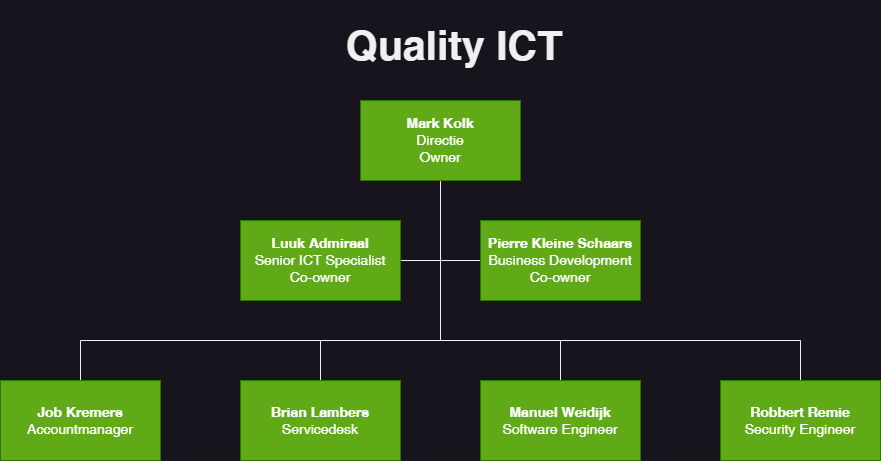
\includegraphics[width=1.0\textwidth]{Figures/OrganizationalDiagram_QICT.png}
      \caption{Flat (hierarchical) structure of \acrshort{qict}, along with its departments and their managers.}
\end{figure}

% \subsubsection{Working Methodology}
% The company currently utilizes the five functions defined by \acrshort{nist} as part of its \acrshort{csf} as
% the framework to help the company manage and improve their cybersecurity risk management processes. These five
% functions are part of the \acrshort{fips} 199. All functions serve as level categories for organizing
% cybersecurity activities within an organization and are as follows (\cite{nist}):
% \begin{itemize}
%       \item \textbf{Identify}: develop the organizational understanding to manage cybersecurity risk to
%             systems, assets, data, and capabilities. This includes the development of an organizational
%             understanding to manage cybersecurity risk to systems, assets, data, and capabilities. It also
%             includes the development of a cybersecurity risk management strategy that is aligned with the
%             organization's mission, goals, and objectives and the establishment of a governance structure to
%             ensure that the strategy is effectively implemented and maintained.
%       \item \textbf{Protect}: develop and implement the appropriate safeguards to ensure delivery of critical
%             infrastructure services. It can help the company assists clients in implementing security controls,
%             encryption mechanism, access controls, and other security measures to protect their systems and
%             data from unauthorized access, disclosure, and alteration or modification.
%       \item \textbf{Detect}: develop and implement the appropriate activities to identify and detect the
%             occurrence of a cybersecurity event in timely manner to facilitate rapid response and mitigation
%             efforts. This includes the development of a cybersecurity event detection capability that is
%             integrated with the company's incident response and recovery capabilities. It will help the
%             company to implement monitoring and detection mechanisms, such as intrusion detection systems,
%             log analysis tools, and \acrshort{siem} systems, to detect and identify to cybersecurity incidents
%             promptly.
%       \item \textbf{Respond}: develop and implement the appropriate activities to act in responding
%             regarding a detected cybersecurity event, containing the impact, and restoring normal operations.
%             It involves activities such as developing incident response plans, conducting incident response
%             drills and exercises, establishing communication channels with stakeholders, and implementing
%             recovery strategies to minimize the impact of cybersecurity incidents on business operations and
%             services.
%       \item \textbf{Recover}: develop and implement the appropriate activities to maintain plans for
%             resilience and to restore any capabilities or services that were impaired due to a cybersecurity
%             incident and event, along with implementing improvements to prevent future incidents. In this
%             activity,  the company should be able to develop and implement recovery plans, conduct
%             post-incident reviews and analysis, identify areas for improvement, and implement measures and
%             improvements to enhance resilience and prevention future incidents.
% \end{itemize}

% \begin{figure}[htbp]
%       \centering
%       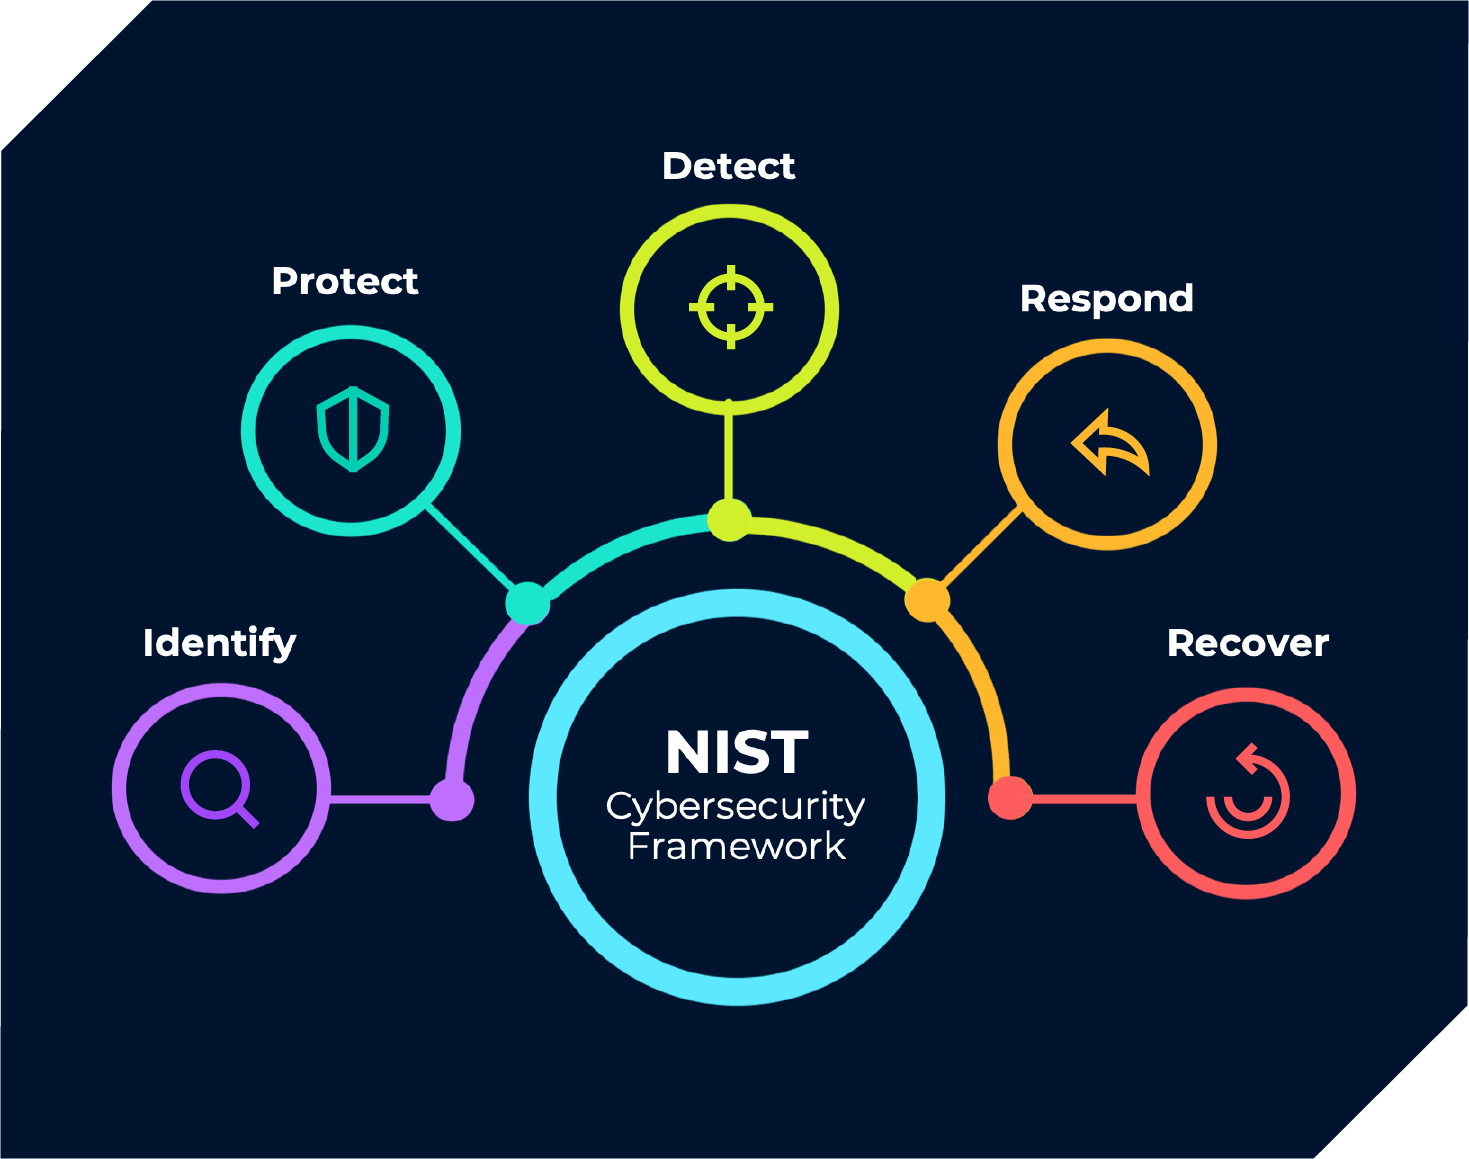
\includegraphics[width=0.8\textwidth]{Figures/qict-working-method.png}
%       \caption{\acrshort{nist} working methodology that is followed by \acrshort{qict}}
% \end{figure}

\subsubsection{Unofficial Partnerships}

\acrshort{qict} has several unofficial partnerships with other organizations, they are normally located in the same building that
\acrshort{qict} rents its office from. These organizations help \acrshort{qict} in their own speciality, and \acrshort{qict} helps them
in return. These organizations are:

\begin{itemize}
      \item MemoICT: is a Shopware company that helps with e-commerce.
      \item Ondernemend Emmen: helps with international entrepreneurship, knowledge sharing, and networking.
      \item Peat Digital: helps with online marketing to promote \acrshort{qict} products more into wider audience.
      \item Webba: helps with web development, especially designing \acrshort{qict}, \acrshort{mkb}iT, and \acrshort{qaas}.nu website.
      \item InDiv Solutions: also helps \acrshort{qict} with the front-end side of their website development.
      \item Pax8: is another official \acrshort{ms} official partner that resell \acrshort{ms} subscriptions and products. It is a
            company based in \acrshort{uk} that helps \acrshort{qict} with their clients manage their subscriptions.
\end{itemize}

Recently, as since of last year, \acrshort{qict} has obtained the rights to the SentinelOne environment and official sell its subscription
to \acrshort{qict} customers under their own name. \acrshort{qict} will then act as the management of the client's domain in SentinelOne
that subscribes to them through \acrshort{qict}. Because SentinelOne is relatively new to the \acrshort{qict}, it has not fully integrated
with the internal system yet. This will be discussed further in the Problem Statement section.

\subsubsection{Internal System and Tools}

\textbf{The QaaS App}

The \acrshort{qaas} app is web application that is used by \acrshort{qict} and its clients.
For \acrshort{qict}'s clients, it is a \acrshort{saas} that is used to see what kind of information are available
regarding their \acrshort{ict} infrastructure, based on the subscriptions that they have with \acrshort{qict}.
For example, a customer that subscribes on N-Central and SentinelOne will be able to see the status of their
devices from N-Central \acrshort{api}, and the health of their devices from SentinelOne \acrshort{api}.
For \acrshort{qict} employees themselves, it serves as an internal system that is used to manage the clients and their
\acrshort{ict} infrastructure.

\begin{figure}[H]
      \centering
      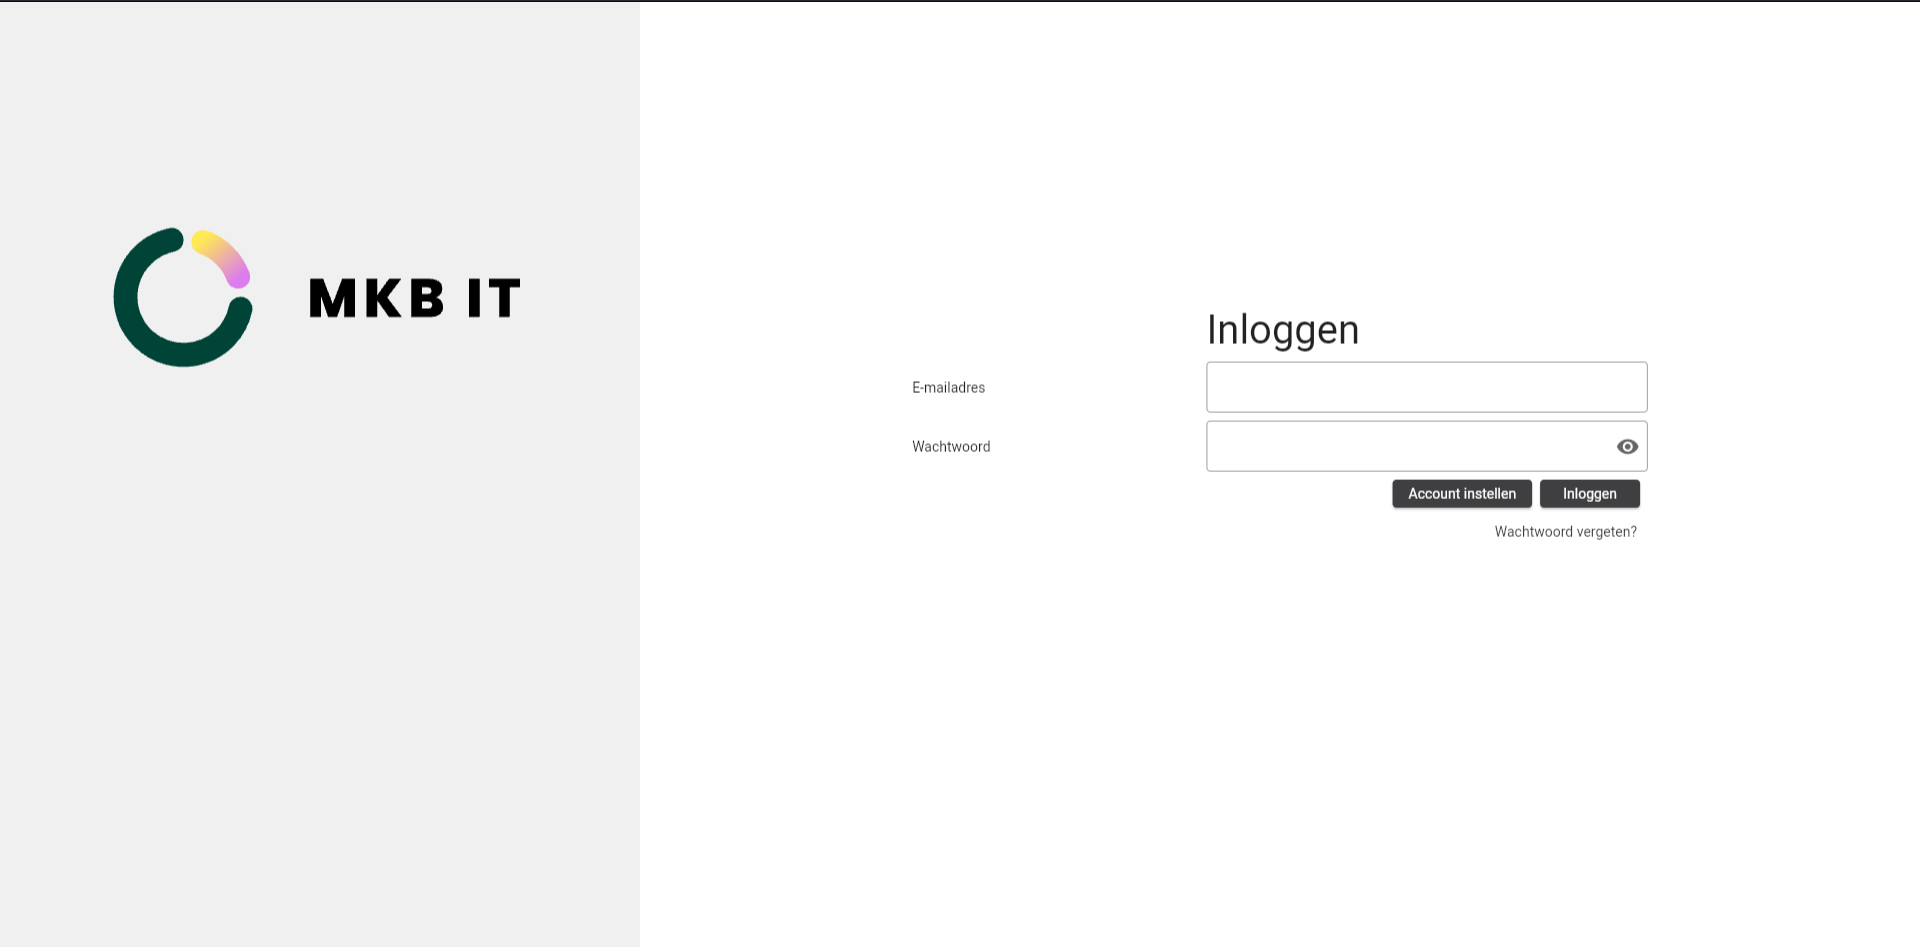
\includegraphics[width=1.0\textwidth]{Figures/Qaas App/Landing Page.png}
      \caption{The login page of the \acrshort{qaas} app, implementing Google \acrshort{2fa} and re\acrshort{captcha}}
\end{figure}

\textbf{APIs and Tools}

The \acrshort{qaas} app also utilizes several \acrshort{api}s and technologies to help with its operations.
It needs to manage and make connection different sort of \acrshort{api}s to help with the operations as an
\acrshort{erp} application. Those \acrshort{api}s are the following:
\begin{itemize}
      \item Resello: is used for \acrshort{qict}'s \acrshort{ms} subscriptions owned by Pax8 (\textit{\cite{resello}}).
            It is a cloud marketplace that simplifies the way \acrshort{sme} companies buy, sell, and manage cloud solutions
            through automation. It provides a single platform to manage the entire cloud customer lifecycle, from
            quote to cash to support, thus simplifying the process of buying, selling and managing cloud
            solutions. Furthermore, it normally uses \gls{SOAP API} for its communication.
      \item SnelStart: is used for \acrshort{qict} automation of financial and accounting system software,
            such as managing invoices, \acrshort{etc} for \acrshort{sme}s. It offers a range of products and
            services to help businesses manage their finances, including accounting software, invoicing software, and financial management
            tools.
      \item Bodyguard.io: is a \acrshort{cdr} tool used for security tab. It is a product from a Dutch company
            that filters and scrutinizes downloads from web browsers to detect and prevent malicious files with
            real-time download scanning capabilities. It normally uses \gls{RESTful API} for its communication.
      \item N-Central: is a product from N-Able and is used for monitoring clients' devices and ensuring the
            overall security of their systems, \acrshort{it} infrastructure, and digital assets. It is a
            \gls{RMM} platform designed to help \acrshort{msp} and \acrshort{it} professionals to
            remotely monitor and manage their clients' devices and networks. It provides a comprehensive
            set of tools and features for monitoring, managing, and securing clients' devices and networks,
            including patch management, \acrshort{av}, backup and disaster reovery, virus scanner,
            network topology mapping, disk encryption, and Windows update that supports showing \acrshort{os},
            disk, and status update. The return response from this \acrshort{api} is in \gls{XML}
            and \acrshort{json} format, making it both a \gls{REST gls} and \acrshort{soap} \acrshort{api}.
      \item PerfectView: is used for \gls{CRM} software (\textit{\cite{perfectView}}). It is designed to
            improve business relationships with customers, assist in customer retention, and drive sales growth.
            In the \acrshort{qaas} app, it is used to manage the relationships and interactions with the app's users,
            which could include tracking user interactions, managing customer support requests and analyzing user
            data to improve the app's functionality and \acrshort{ux}.
\end{itemize}

\begin{figure}[H]
      \centering
      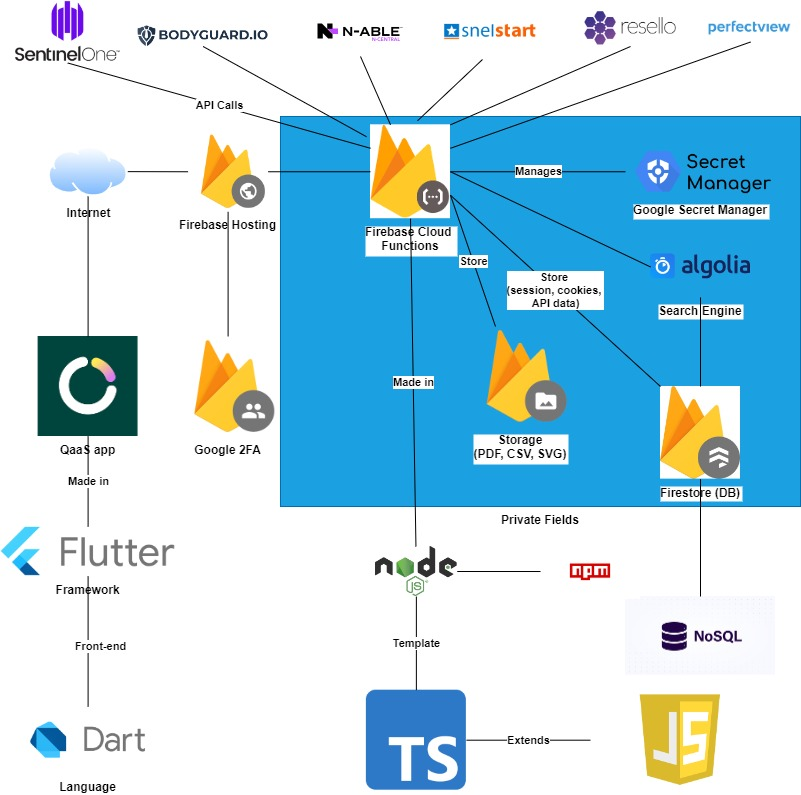
\includegraphics[width=1.0\textwidth]{Figures/QaaS App Infraastructure.jpg}
      \caption{The infrastructure of the QaaS app}
\end{figure}

Besides all the 5 internal \acrshort{api}s that \acrshort{qict} uses, the company also uses several technologies to help them with their
operations. Those tools are:

\begin{itemize}
      \item Computicate (now newly named Acronis): is used as their ticketing system, providing ticketing solution services to customers for
            a wide range of events and activities (\textit{\cite{computicate}}).
      \item TOMTelecom: is used for their company's phone system. It is responsible for structured process of call routing on incoming calls
            from customers to the appropriate department or individuals, ensuring effective communication and issue resolution
            (\textit{\cite{tomTelecom}}).
\end{itemize}

\subsubsection{Subscriptions}

\acrshort{qict} has monthly subscription that it offers to its clients. Subscription within the \acrshort{qict} is divided into smaller
proportions which are the following:
\begin{enumerate}
      \item \acrshort{qaas} Safe: includes security package, patch management, monitoring for workstations or laptop, and traditional
            \acrshort{av} like BitDefender. This traditional \acrshort{av} product will be removed soon as SentinelOne \acrshort{edr} platform
            itself is properly integrated to the \acrshort{qaas} environment since it is already an upgrade from traditional \acrshort{av}. This
            subscription is required for every user in a company to be the official client of \acrshort{qict}. SentinelOne payment subscription
            will also be included in this after the integration.
      \item \acrshort{qaas} Safe+: for advance security protection. Bodyguard.io is included. This subscription is still a proof of concept
            within the stakeholders.
      \item \acrshort{qaas} Help: is used for a free call service to the helpdesk between working hours (Monday to Friday, 08:30 - 17:00).
            This subscription will utilize external tracking system to check whether a user has this subscription to ensure proper billing.
            Then a financial and ticketing system like SnelStart and Computicket is used for billing users who call the Helpdesk who do
            not have this subscription.
      \item \acrshort{qaas} Back-up: for back-ups from the data of the customer from MS 365 Cloud provider. It is for restoring if data is
            lost. The data will be stored off-site in OneDrive as the cloud personal storage since \acrshort{qict} is a Microsoft partner.
            This subscription has also a collaboration with N-Central for its back-up and disaster recovery solutions.
\end{enumerate}


% \subsubsection{Q-ICT Sister Companies}

% \acrshort{qict} has 2 other sister companies who are also under the same ownership of Mark Kolk, which are \acrshort{mkb}iT and
% \acrshort{qaas}.nu respectively.

% \textbf{MKBiT}

% It is a parent-company of \acrshort{qict} who provides IT solutions and consultation to its clients. It was founded to support
% \acrshort{qict} business operations. It shares the same office with \acrshort{qict}. Its services include cloud solution, Microsoft 365
% products, patch-management, online-backup, \acrshort{av}, anti-spam, and monitoring software applications.

% Luuk Admiraal is directing this company. Because the company is an \acrshort{it} service provider, it has a vast network of suppliers and
% partners to provide them with the products and brands to support their business. Here is the list of the suppliers:
% DrayTek, HP, Microsoft, and Ubiquiti Network.

% \textbf{QaaS.nu}

% This company is responsible for the software development of \acrshort{qict}. It is still a small company which was set up not a while ago,
% so there is not a lot of info feasible for the author to write about it. Their upcoming projects are still proof-of-concept. The company
% is directed by Pierre Kleine Schaars. This terminology is not to be confused with the \acrshort{qaas} app, which is the internal app of
% all the three companies.

% \begin{figure}[htbp]
%       \centering
%       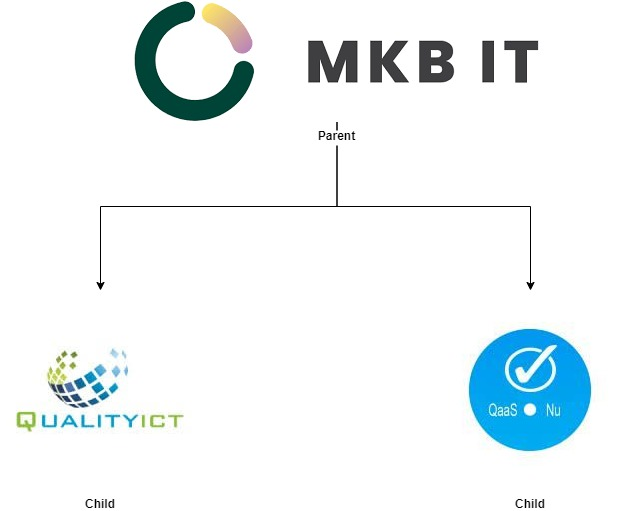
\includegraphics[width=1.0\textwidth]{Figures/q-ict.jpg}
%       \caption{The relation between the three companies}
% \end{figure}

\subsubsection{Products and Services}

% Besides cybersecurity, together with \acrshort{mkb}iT and \acrshort{qaas}.nu, \acrshort{qict} offers a wide range of products and
% services to its clients. Those products are (\textit{\cite{qictProducts}}):

Some products of \acrshort{qict} are already discussed briefly in the subscription section. But here are the full review:

\begin{itemize}
      \item Customized software development: this field is one of the main responsibilities of \acrshort{qict} itself, it provides
            customers with tailor-made software solutions that are designed to meet their specific needs and requirements. The company
            works closely with clients to understand their unique challenges and develop software applications that effectively address
            those concerns.
      \item Online-backup: the company offers a service where the clients can store copies of their files, documents, and data on remote
            servers via the internet. These remote servers are hosted in secure data centres. Furthermore, \acrshort{mkb}iT also provides
            \acrshort{db} migration in case any event of disasters occurred.
      \item Active monitoring: the company will offer its customers the chance to oversee, track, and manage their computer systems,
            networks, or applications in real-time. It serves various purposes, including ensuring system stability, optimizing
            performance, enhancing security, and providing valuable insights into the usage patterns and behaviours of users or devices.
            In the future, it wants to bring more automation to its system, providing customers with automatic messages when a disk space
            becomes full, or when there is an error message in clients' computers.
      \item Anti-spam software: a specific type of software application that is designed by \acrshort{mkb}iT to detect, prevent, and block
            unsolicited and unwanted e-mail messages, commonly known as spam, from reaching clients' e-mail inboxes. They are typically
            sent in bulk to many recipients without their consent, often containing advertisements, phishing attempts, malware, or other
            malicious content. It has features such as whitelist, blacklist, and filter e-mails per e-mail account or e-mail address.
      \item Microsoft 365 products: the company is also providing access to Microsoft's suite of cloud-based productivity tools and
            services, including installation services, to its clients. These include Microsoft Word, Excel, PowerPoint, Outlook, and more,
            which are all accessible online through a web browser or can be installed on local devices such as computers and smartphones.
      \item \acrshort{av} software: it resells and gives clients advice and comparisons on good antivirus software from manufacturers like
            McAfee and Bitdefender. This software is designed to detect, prevent, and remove malware from computer systems.
      \item Cloud services: the company also provides clients with a tailor-made cloud solution based on their specific wishes and
            problems, whether it is using a public, private, or hybrid cloud. It delivers a range of computing resources, applications,
            and services over the internet through cloud computing technologies. These services enable the clients to access and use
            computing resources without the need to own or maintain physical hardware and software infrastructure, enabling their
            employees to access their files anytime, anywhere, without others having to access them.
\end{itemize}

In addition, for the software development, \acrshort{qict} also uses other \acrshort{ms} technologies such as Power Platform
(\acrshort{ie} Power Automate, Power BI, Power Apps, Power Virtual Agents, and Power Pages), Dynamics 365, and Azure to help with their
software development, therefore the clients who are asking for the product to be developed with the help of  those \acrshort{ms}
technologies will also have those subscriptions of the products, therefore paying extra charge.

\section{Problem Statement}
The company currently manages numerous third-party \acrshort{api}s mentioned above for various purposes.
Currently, the company has already offered SentinelOne endpoint protection subscription to its clients.
However, the clients cannot access to SentinelOne dashboard without \acrshort{qict} making the
necessary accounts for every single individual first. Making the accounts for the clients can be a time-consuming process,
seeing that the clients reach up to 400 active companies, therefore an integration of SentinelOne
to \acrshort{qict}'s own internal system is more advantageous to the company by allowing clients to see
their SentinelOne data related to their system and endpoint health directly through \acrshort{qict}'s
platform. Moreover, it is not beneficial from a business perspective to direct customers to other external
security solutions, as most of the data in SentinelOne is in English and \acrshort{qict} want to be the
primary resource for cybersecurity assistance for its clients around the Netherlands.

Furthermore, the SentinelOne dashboard is not user-friendly to the clients. It is made to directly assist cybersecurity
specialist like threat analysts working in \acrshort{soc} department or \acrshort{it} administrators. Therefore,
\acrshort{qict} also wishes that this integration to be designed as user-friendly as possible, considering
that most clients have limited or no knowledge at all about cybersecurity or computers. Thus, the integration of SentinelOne to the
\acrshort{qaas} App simply adds a layer of functionality to the clients, enabling them to see and easily
understand the data. In essence, SentinelOne will complement the \acrshort{qaas} app by providing enhancement to the
app so that it can show, visualize and display the intricate data related to endpoint security such as real-time insights,
comprehensive audit trails, threat intelligence, endpoint security logs, configuration details, user activity logs, telemetry data,
alerts, remediation actions, reports and analytics, and more. This will then add more value to the \acrshort{qaas} App as an advance
threat detection platform providing user-friendly security dashboard that offers detailed insights into device health and status. This
project will not however, make any changes related to how the internal system architecture of SentinelOne, including the structure of
its Agents and the algorithms driven by \acrshort{ai} and \acrshort{ml}.

By this integration, the \acrshort{qaas} App will also complement SentinelOne by promoting it to the broader audience, especially here
in the Netherlands. By embedding SentinelOne's advanced security features into the \acrshort{qaas} App, \acrshort{qict} showcases the
robustness and reliability of SentinelOne's solutions to its extensive client base. This integration acts as a powerful endorsement,
demonstrating SentinelOne's effectiveness in real-world scenarios and highlighting its value in providing comprehensive cybersecurity
protection.

Thus, the company has tasked the author with the development of the SentinelOne security threat platform
integration for continuous cybersecurity monitoring within the \acrshort{qaas} app as the main topic of his
graduation work  placement project.

\section{Project Objectives}
In the end of this project which consist of 90-99 working days, the following objectives should be achieved:
\begin{enumerate}
      \item Effectively integrates and leverages the SentinelOne \acrshort{edr} platform for continuous
            cybersecurity monitoring within the \acrshort{qaas} app.
      \item The \acrshort{qaas} app should have a way to visualize the data retrieved from the SentinelOne
            \acrshort{api} in a user-friendly manner in order for the client users helpdesk support, financial
            department, cybersecurity department, software development department, and other employees within
            \acrshort{qict}  departments to see the data easier.
            %     \item Combine the SentinelOne data with N-Central \acrshort{api}
            %     \item Utilize Vigilance package of SentinelOne
            %     \item Ensure proper unit testing, code refactoring, commenting, and adherence to the overall code
            %           conventional guidelines and best practices in both the test and live environments of the
            %           \acrshort{qaas} app.
\end{enumerate}
\section{Reading Guide}
This report is structured as follows:
\begin{itemize}
      \item \textbf{Summary}: provides a brief and concise overview of the entire report, including the
            research questions, key findings, and conclusion. Its purpose is to provide readers with a
            quick and comprehensive understanding of the report.
      \item \textbf{Introduction}: provides an overview of the project background, the research topic of the
            company, and the project objectives. It introduces the context of the research and outlines the
            structure of the report.
      \item \textbf{Research Design}: outlines the methodologies employed during the research
            process. It describes the research approach, data collection methods, selected measuring instruments,
            data analysis techniques used to address the research questions, reliability, validity, and general
            applicability.
      \item \textbf{Research Results}: presents the research results, including the research methodology, the findings,
            and the analysis of the research questions. Firstly, it describes the methodologies employed
            during the research, and then it provides a detailed account of the research process and the
            outcomes of the research.
      \item \textbf{Realization}: provides a detailed description of the software end-product developed during
            this work placement project. It outlines insights into design, development, and implementation
            phases. It also highlights key features, functionalities, and technology specifications used in
            the project.
      \item \textbf{Conclusions and Recommendations}: the Conclusion summarizes the key findings and results
            achieved during the research and realization phases. The Recommendation section outlines the
            proposed next steps and future research areas to further enhance the project and address any
            outstanding issues. It discusses potential areas for further exploration or refinement.
      \item \textbf{References}: lists all the sources cited in the report following the appropriate to
            \acrshort{apa} 7th edition citation style.
      \item \textbf{Appendices}: includes any additional supplementary information, data, or materials that
            are relevant to the report but not included in the main body of the report.
\end{itemize}

\chapter{Research Results}
\begin{multicols}{2}
    In a research, it is paramount to have the formulation of a clear research topic, research main question, and research
    sub-questions. The main question serves as the focal point around which the researchr revolves, encapsulating the primary
    objective or purpose of the study. The research sub-questions are then used to function as a pathway that dissect
    The following main research question will be use throughout the research:
    \begin{center}
        \textit{"How can Q-ICT effectively enhance API monitoring within its internal application while integrating
            and leveraging SentinelOne security threat platform for continuous cybersecurity monitoring while
            still ensuring adherence to the highest security standards?"}
    \end{center}
    The research main question is then expanded in the following research sub-questions:
    \begin{itemize}
        \item What is the current situation of the QaaS app of Q-ICT?
        \item How can SentinelOne can be integrated into the QaaS app environment, especially aligning with the
              \acrshort{api} monitoring functionality, while still utilizing their key features and capabilities in
              context of cyber threat detection and remote IT infrastructure management?
    \end{itemize}
    \section{Research Methodology}
    In this research, different research methods have been used to answer the research questions. This research will
    based on the six \acrshort{ict} research methods defined by HBO-I (\cite{ictresearchmethods}). A research method for
    each sub-question is then defined along with how the results are considered valid and reliable:
    \begin{itemize}[label=-]
        \item Sub-question \#1:
        \item Sub-question \#2:
        \item Sub-question \#3:
        \item Sub-question \#4:
    \end{itemize}
    \section{Research Question \#1: What is the Current Situation of the QaaS App of Q-ICT?}
    The \acrshort{qaas} app is a web application that is used by \acrshort{qict} .
    \subsection{QaaS App Infrastructure}
\end{multicols}
\chapter{Realization}

\begin{multicols}{2}
  Because the \acrshort{qaas} web application itself is already built on top of existing frameworks, libraries, and technologies, the integration of the SentinelOne
  was relatively straightforward. The \acrshort{api} itself is well-documented, and the \acrshort{npm} package provided by SentinelOne is easy to use. The only challenge
  was to understand the data structure of the SentinelOne, choosing the right and more important data to display, modelling it in the \acrshort{qaas} database, and then
  displaying it in the web application.

  \section{The Back-end}

  As stated before, \acrshort{qict} wishes to utilize the 2nd generation of Firebase Cloud Functions, therefore a new Firebase project was created and stored on the cloud
  (\textit{using Azure DevOps}). The author also needs to make a decision in regards on how the infrastructure of the codebase should be structured. Because \acrshort{qict}
  is always critical and open to feedback, the author is given access to the old Firebase codebase (\textit{utilizing version 1.0}), and find any potential upsides and
  downsides of that project repository. The author then, by an informed decision, is allowed to decide whether to structure the new codebase in the same way as the old one.
  The author has certainly decided to create some new adjustments to the new codebase. For example, instead of stacking all functionalities that a Firebase Cloud Function
  might have, the author has decided to improve the codebase especially regarding the separation of concerns. Specifically, the response from the \acrshort{api} is
  modelled using Interfaces and Classes object within the Models directory, allowing for a consistent reuse across different functions. Additionally, distinct Routers and Controllers
  directories has been established, each with specific responsibilities. The Routers directory primarily handles external communications with the \acrshort{api},
  utilizing \texttt{Axios} (\textit{\cite{axiosNpm}}) for handling the GET requests. The Controllers directory, contains the back-end logic of the cloud function,
  bridging Models and Routers and ensuring comprehensive error documentation. This structure defines the behavior of the Firebase Cloud Function version 2.0 of the
  \acrshort{qaas} app.

  Moreover, there are Utilities and Middlewares directories, which are used to handle common functionalities and errors. The Utilities directory contains functions that
  are used across the codebase, such as logging errors, and the Middlewares directory contains functions that are used to handle the request and response of the
  cloud function. For example, the \texttt{logError} function in the Utilities directory is used to log errors in the console, and the \texttt{handleError} function in
  the Middlewares directory is used to handle errors in the response of the cloud function. This structure allows for a more organized and maintainable codebase.

  The types of functions that are used throughout the project are the following:
  \begin{itemize}
    \item \texttt{onCall}: This type of function is used to handle callable functions, which are called from the client-side. It is used to handle requests from the
          client-side. This is the main function in which the SentinelOne data is fetched and processed.
    \item \texttt{onRequest}: This type of function is used to handle \acrshort{http} requests, which are called from the client-side. It is mainly for initial testing, as
          setting this function up is easier and faster. However, the author does not recommend using this in the production, as it lacks authentication and security
          for the end-user.
    \item \texttt{onSchedule}: This type of function is used to handle scheduled functions, normally called cron-jobs, which are called at a specific time. It is used
          to handle scheduled tasks that need to be executed at a specific time. There is only one scheduled function in the project, which is used to replace the old
          SentinelOne \acrshort{api} key with a new one that is securely stored in Google Secret Manager, therefore ensuring proper connection and access to the secret
          vault, every month.
  \end{itemize}

\end{multicols}


\begin{lstlisting}[language=JavaScript, caption={An example of Firebase HTTP Request onCall Cloud Function version 1.0}]
  import * as functions from "firebase-functions";
  import * as admin from "firebase-admin";
  import { Secrets } from "../Firebase/Secrets";
  import { FirebaseCall } from "../Firebase/FirebaseCall";
  import axios from 'axios'; 

  export default functions
    .region("europe-west1")
    .https.onCall(async (data, context) => {
        try {
          // context.app will be undefined if the request doesn't include a valid
          // App Check token.
          if (context.app === undefined) {
            throw new functions.https.HttpsError(
              "failed-precondition",
              "The function must be called from an App Check verified app."
            );
          } 
        } catch (error) {
          console.error("An error occurred in the Firebase HTTP Request onCall Cloud Function: ", error);
          throw new functions.https.HttpsError("internal", "An error occurred while processing the request.");
        }
  });
\end{lstlisting}

\begin{lstlisting}[language=JavaScript, caption={onCall Cloud Function version 2.0, where the parameters of the function is less and the way it handles the authorization is different}]
  import axios from "axios";
  import * as functions from "firebase-functions/v2";
  import { CallableRequest } from "firebase-functions/v2/https";
  import admin from "firebase-admin";

  import { region, sentinelOneURL, sentinelOneApiVersion } from "../../../config";
  import { logError } from "../../../Middleware/LogError";
  import { getSecret } from "../../../Util/Secret";

  export const getSentinelOneData = functions.https.onCall({ region: region }, async (context: CallableRequest<any>) => {
    try {
      // Authentication check
      if (!context.auth) {
        throw new functions.https.HttpsError("unauthenticated", "The function must be called while authenticated.");
      }
      const data = context.data;
  
      // // Checking if the request contains the necessary data
      if (!data || !data.siteId || !data.userId || !data.dataType) {
        throw new functions.https.HttpsError("invalid-argument", "The necessary requirement(s) are missing or invalid in your request.");
      }  
    } catch(ex: unknown) {

    }
  });
\end{lstlisting}

\begin{lstlisting}[language=JavaScript, caption=LogError functionality in the Utilities folder]
  export function logError(error: unknown, context: string): void {
    if (isAxiosError(error)) {
      // AxiosError object, log detailed request and response information
      console.error(`[${context}] Axios error occurred: ${error.message}`);
      console.error(`Response data: ${error.response?.data}`);
      console.error(`Status code: ${error.response?.status}`);
      console.error(`Headers: ${JSON.stringify(error.response?.headers, null, 2)}`);
    } else if (error instanceof Error) {
      // Standard Error object, log message and stack
      console.error(`[${context}] An error occurred: ${error.message} \n Stack: ${error.stack}`);
    } else {
      // Non-Error object, log with a generic message
      console.error(`[${context}] An unknown error occurred:`, error);
    }
  }
\end{lstlisting}


\begin{lstlisting}[language=JavaScript, caption={An example of how that utility is used in the Cloud Function, the reasong why exception type is unknown is to comply with the ESLint rules that does not recommend to use the any type to the variables}]
  try {

  }
  catch (ex: unknown) {
    console.log(`An error occured in the getFirestoreData function: ${ex}`);
    logError(ex, "getFirestoreData");
  } finally {
    throw new functions.https.HttpsError("internal", "An error occurred while getting the data in Firestore.");
  }
\end{lstlisting}

\begin{multicols}{2}
  \subsection{SentinelOne NPM package}

  \subsection{Compliance with ESLint compiler}
  \acrshort{js} in nature is a loosely typed language, and it is easy to make mistakes in the code as its variables do not have a fixed type. While this sometimes can be
  beneficial as it makes the development faster and more flexible, it also introduces challenges, particularly in debugging and maintaining the code. To prevent this,
  both the author and the Company Supervisor have decided to use and adhere to \acrshort{ts} and ESLint rules, to ensure static typing, code quality
  and consistency to the coding standards.
\end{multicols}


\begin{lstlisting}[language=JavaScript, caption={Example of challenges in JavaScript because of its loosely typed nature that creates lack of type safety, type coercion, and type conversion}]
  function add(a, b) {
    return a + b;
  }
  console.log(add(5, '2')); // "52" instead of 7
\end{lstlisting}

\begin{lstlisting}[language=DOS, caption={Another example of JavaScript challenges}]
    C:\Users\ChristopherSulistiyo>node
    Welcome to Node.js v22.1.0.
    Type ".help" for more information.
    > true == 1
    true
    > true === 1
    false
    > true + true + true === 3
    true
    > 0 == "0"
    true
    > "0" ==- null
    true
    > NaN.valueOf()
    NaN
    > -null
    -0
    > 99999999999999999999
    100000000000000000000
    > -0 == "0"
    true
    > parseInt("0.00005")
    0
    > parseInt(0.00000005)
    5

    > let a = []
    undefined
    > a.length == a
    true
  \end{lstlisting}

\chapter{Conclusion and Recommendation}

\begin{multicols}{2}

  \section{Conclusion}
  Cybersecurity is a complex field and threat actors are ever evolving their trade-craft in clever ways. Every single
  running business is not too small to be attacked, but they may be too small for them to make the news. Therefore, transparency
  to the clients is important, because lack of visibility to the clients can lead to a loss of trust. This graduation project serves as the
  first iteration by \acrshort{qict} about the integration of SentinelOne to its internal application, the \acrshort{qaas} app.

  SentinelOne \acrshort{edr} platform is possible to be integrated with the \acrshort{qaas} app, which was made in Flutter with
  Firebase as the back-end cloud solution, utilizing SentinelOne \acrshort{api} to fetch the data. In order that this \acrshort{api}
  to be able to send the correct data, the necessary Agents and Ranger need to be set up properly in a client's machine. This Agent will then serve
  to replace the traditional \acrshort{av}, as it will gather the data from the client's machine and send it to the management \acrshort{db}, providing real-time
  monitoring. Additionally, a SentinelOne account with the necessary rights to read the data with its \acrshort{api} key is also needed to be configured. In the
  front-end, the visualization is done using the Flutter package: \textit{fl\_chart} and \textit{syncfusion\_flutter\_charts}. The \acrshort{qaas} app itself has 3
  different user roles in its system: the clients, the helpdesk, and the \acrshort{it} admins. The objective of this project is that for the \acrshort{qaas} app to
  be used by the clients to see the status of their devices, and the helpdesk and \acrshort{it} admins to manage and monitor the client devices that are connected to
  the SentinelOne \acrshort{edr} platform. For the client user, they can see the status of their devices that are connected to the SentinelOne \acrshort{edr}
  The user itself can customize which charts and data they want to see in the dashboard,
  to make it more user-friendly and catching up with other \acrshort{edr} platforms. The user can also see the details of the
  threats that are detected by SentinelOne, and the user can also see the details of the devices that are connected to the SentinelOne
  \acrshort{edr} platform.

  In the back-end, several functions with different functionalities need to be created to handle the data that is fetched from different SentinelOne
  \acrshort{api} endpoints. The user's session and preference data are stored in the Firebase Firestore \acrshort{db}, and as well as \acrshort{ai} powered
  Algolia search engine to make the search faster and more accurate. Additional features such as filtering, sorting, and pagination will be handled by
  inputting the correct headers to the \acrshort{api} request.

  \section{Recommendation}

  \subsection{Structure of the front-end codebase}

  There are some issues that the author has noticed with the way the \acrshort{qaas} app code was structured. For example, when
  assigning modules to a user,


  \subsection{Integration with N-Central data}

  \subsection{Redis middleware NoSQL database caching}
  Redis is a powerful tool for \acrshort{db} that uses in-memory data structure to provide caching and message broker. It supports various
  data structures (\textit{\cite{redisDataStructure}}), such as strings, hashes, lists, sorted sets, with range queries, bitmaps, hyperlogs,
  geospatial indexes with radius queries, and streams.

  Because the main idea in Redis is to provide caching of the data, coupled with the fact that it is a \acrshort{nosql} \acrshort{db},
  Redis is exceptionally fast to query due to its in-memory nature in contrast to traditional disk-based \acrshort{db}s. This makes it
  suitable for use cases where low latency and high throughput are required, making it perfect for getting and storing data that is frequently
  accessed.

  The idea is to put SentinelOne data into the Redis \acrshort{db} too, with the limit of 5-10 minutes before the cache is deleted, and then fetch
  the data from the Redis \acrshort{db} instead of directly fetching it from Firestore and SentinelOne \acrshort{api} constantly.

  As of April 2024, Redis (\textit{\cite{redisIsNoLongerFree}})

  % Modules issue

  % N-Central API issue: Not all data is correct

  % API monitoring
\end{multicols}


\begin{figure}[htbp]
  \centering
  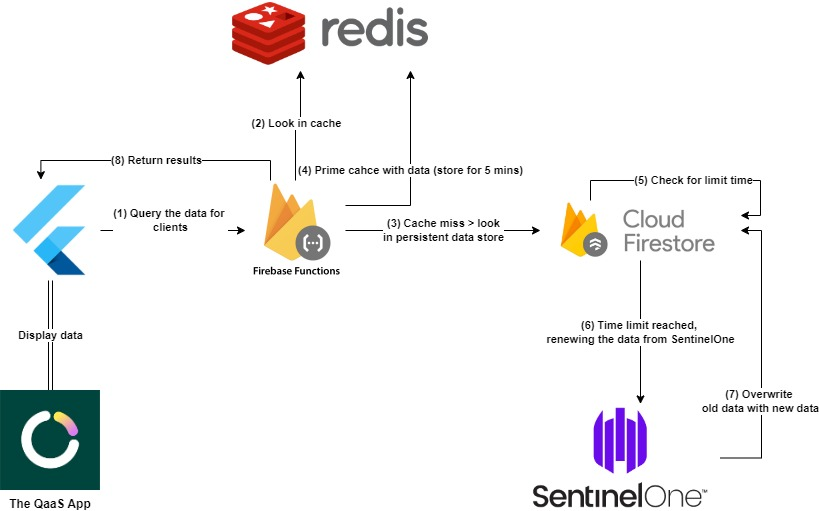
\includegraphics[width=0.8\textwidth]{Figures/Redis Caching.jpg}
  \caption{How the infrastructure would look if Redis is implemented}
\end{figure}
\addcontentsline{toc}{chapter}{Bibliography}
\printbibliography
\appendix

\chapter{FD (Functional Design)} \label{appendix:fd}

\includepdf[pages=-]{AppendixNew/Functional Design.pdf}
\newpage

\chapter{TD (Technical Design)} \label{appendix:technical-design}

\includepdf[pages=-]{AppendixNew/TD.pdf}
\newpage

\chapter{Deployment Manual} \label{appendix:deployment-manual}
\includepdf[pages=-]{AppendixNew/QaaS app deployment manual.pdf}


\chapter{Project Plan} \label{appendix:project-plan}

\includepdf[pages=-]{AppendixNew/Project Plan.pdf}
\newpage

\chapter{Research Proposal}

\includepdf[pages=-]{AppendixNew/Research Proposal.pdf}
\newpage

\chapter{Initial Description of Graduation Project}
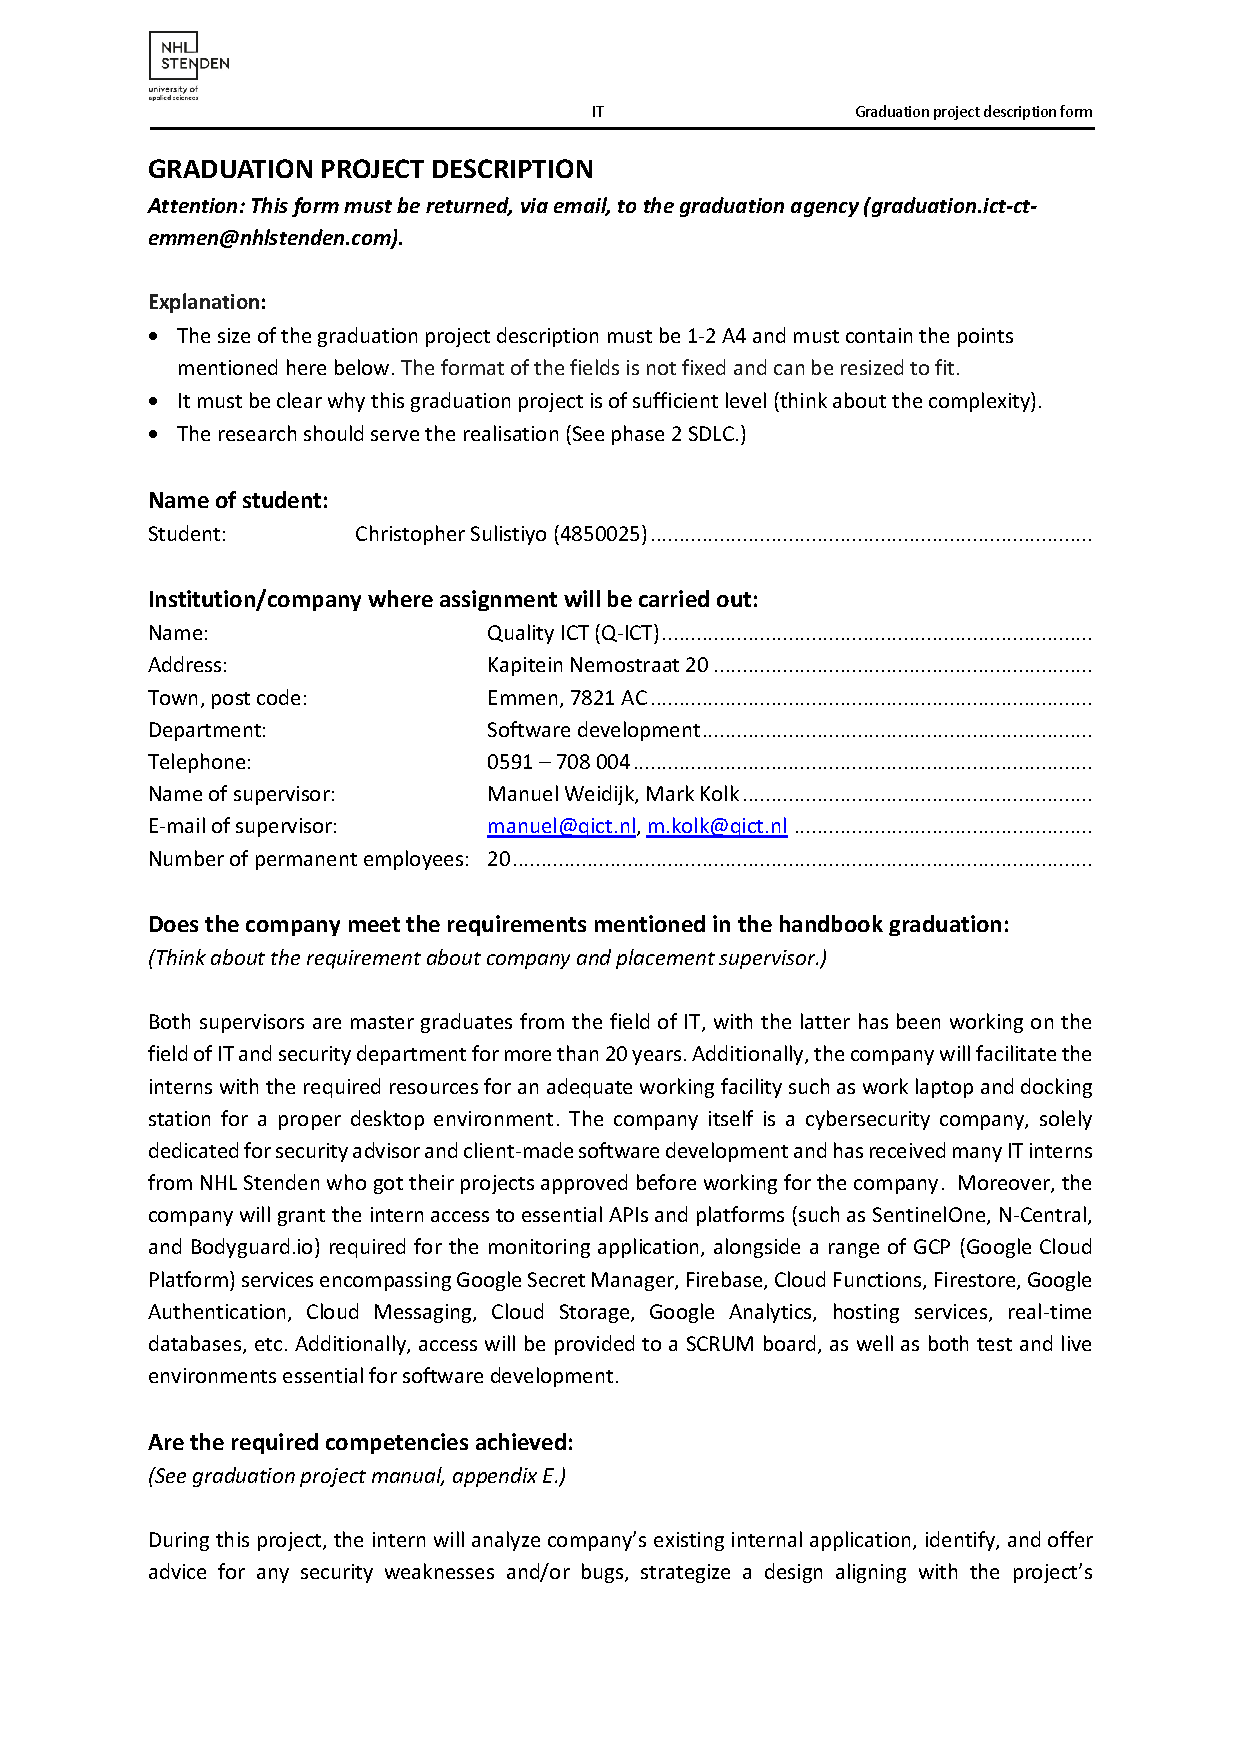
\includepdf[pages=-]{AppendixNew/Initial Description Graduation Project.pdf}
\newpage

% \chapter{SentinelOne API documentation}
% % \includepdf[pages=-]{Appendices/ApiDocs2.1 .pdf}
% \newpage

\chapter{Interview SentinelOne Transcript}
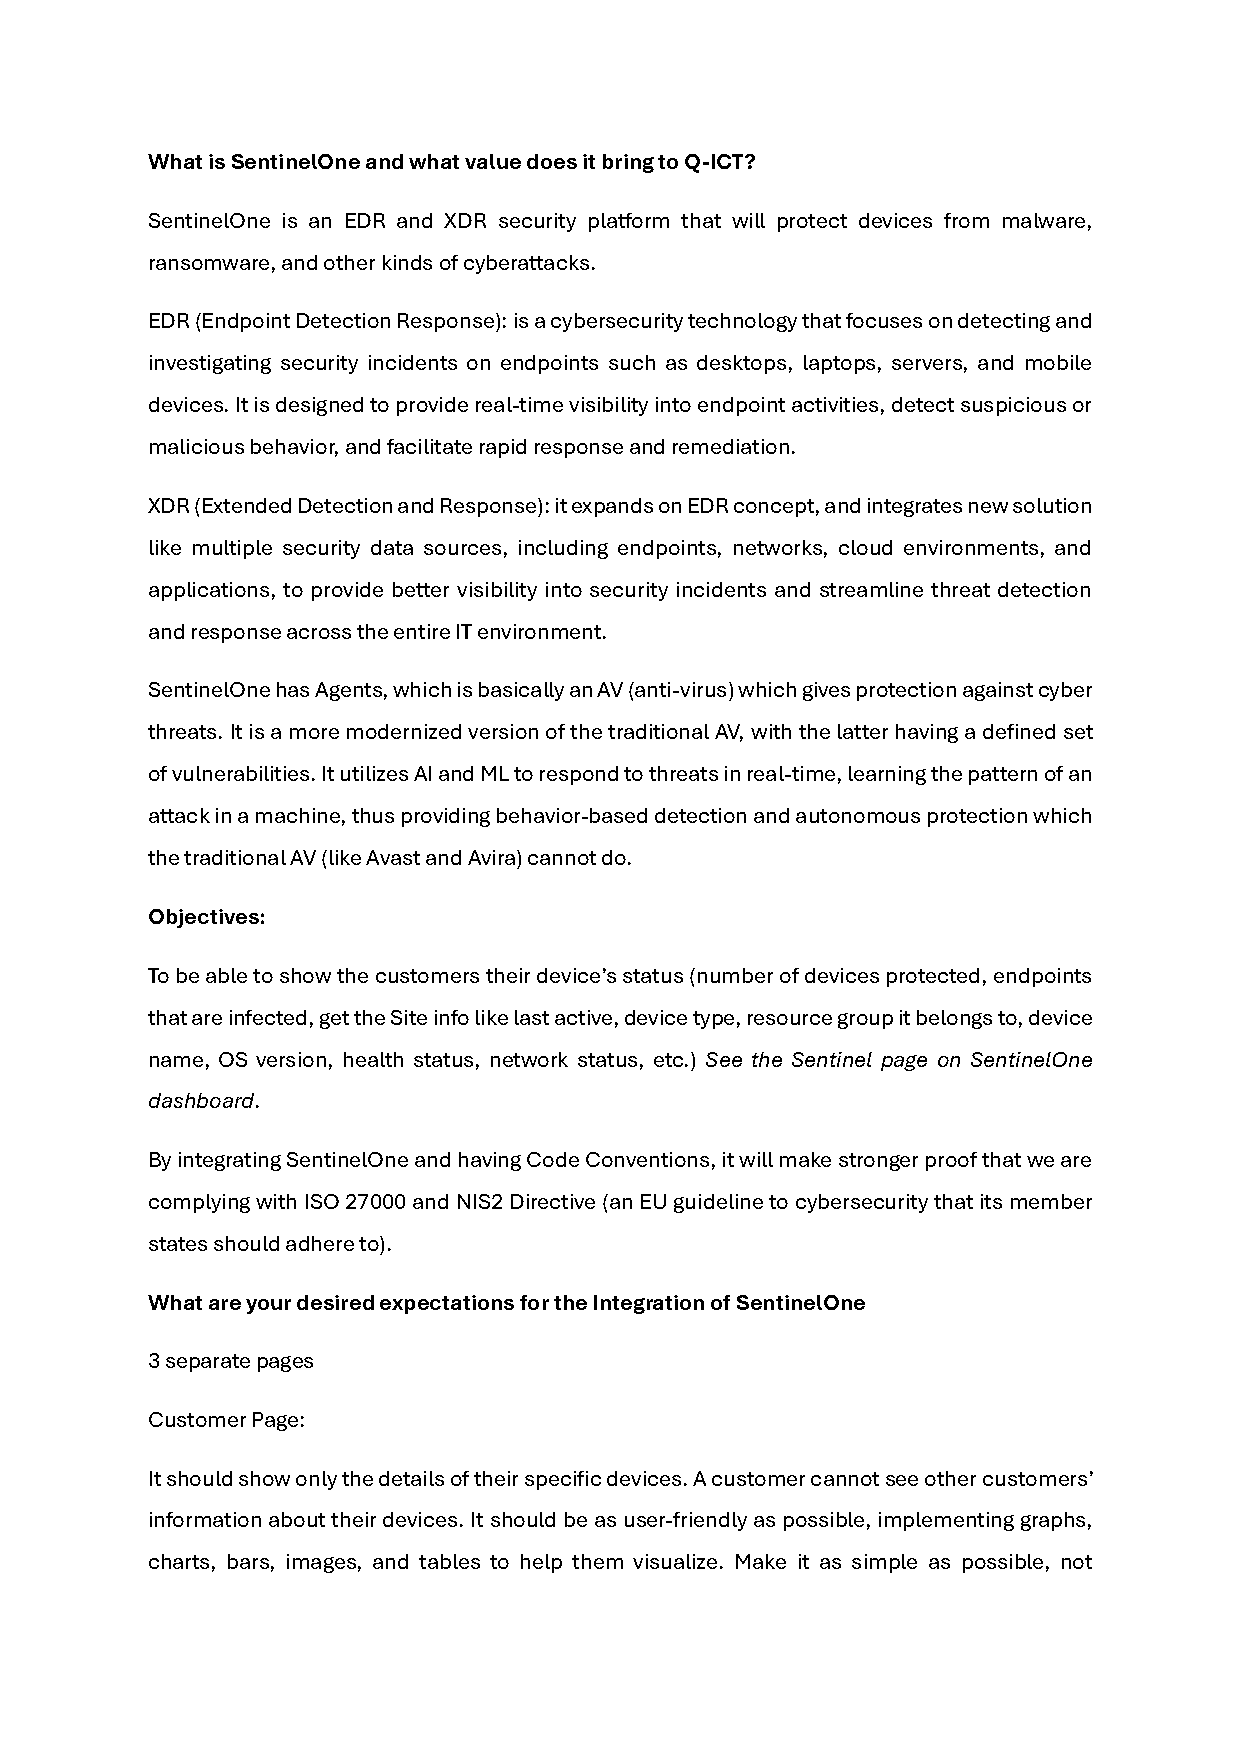
\includepdf[pages=-]{Appendices/SentinelOne Interview Summary.pdf}
\newpage

\chapter{Interview QaaS App Transcript}
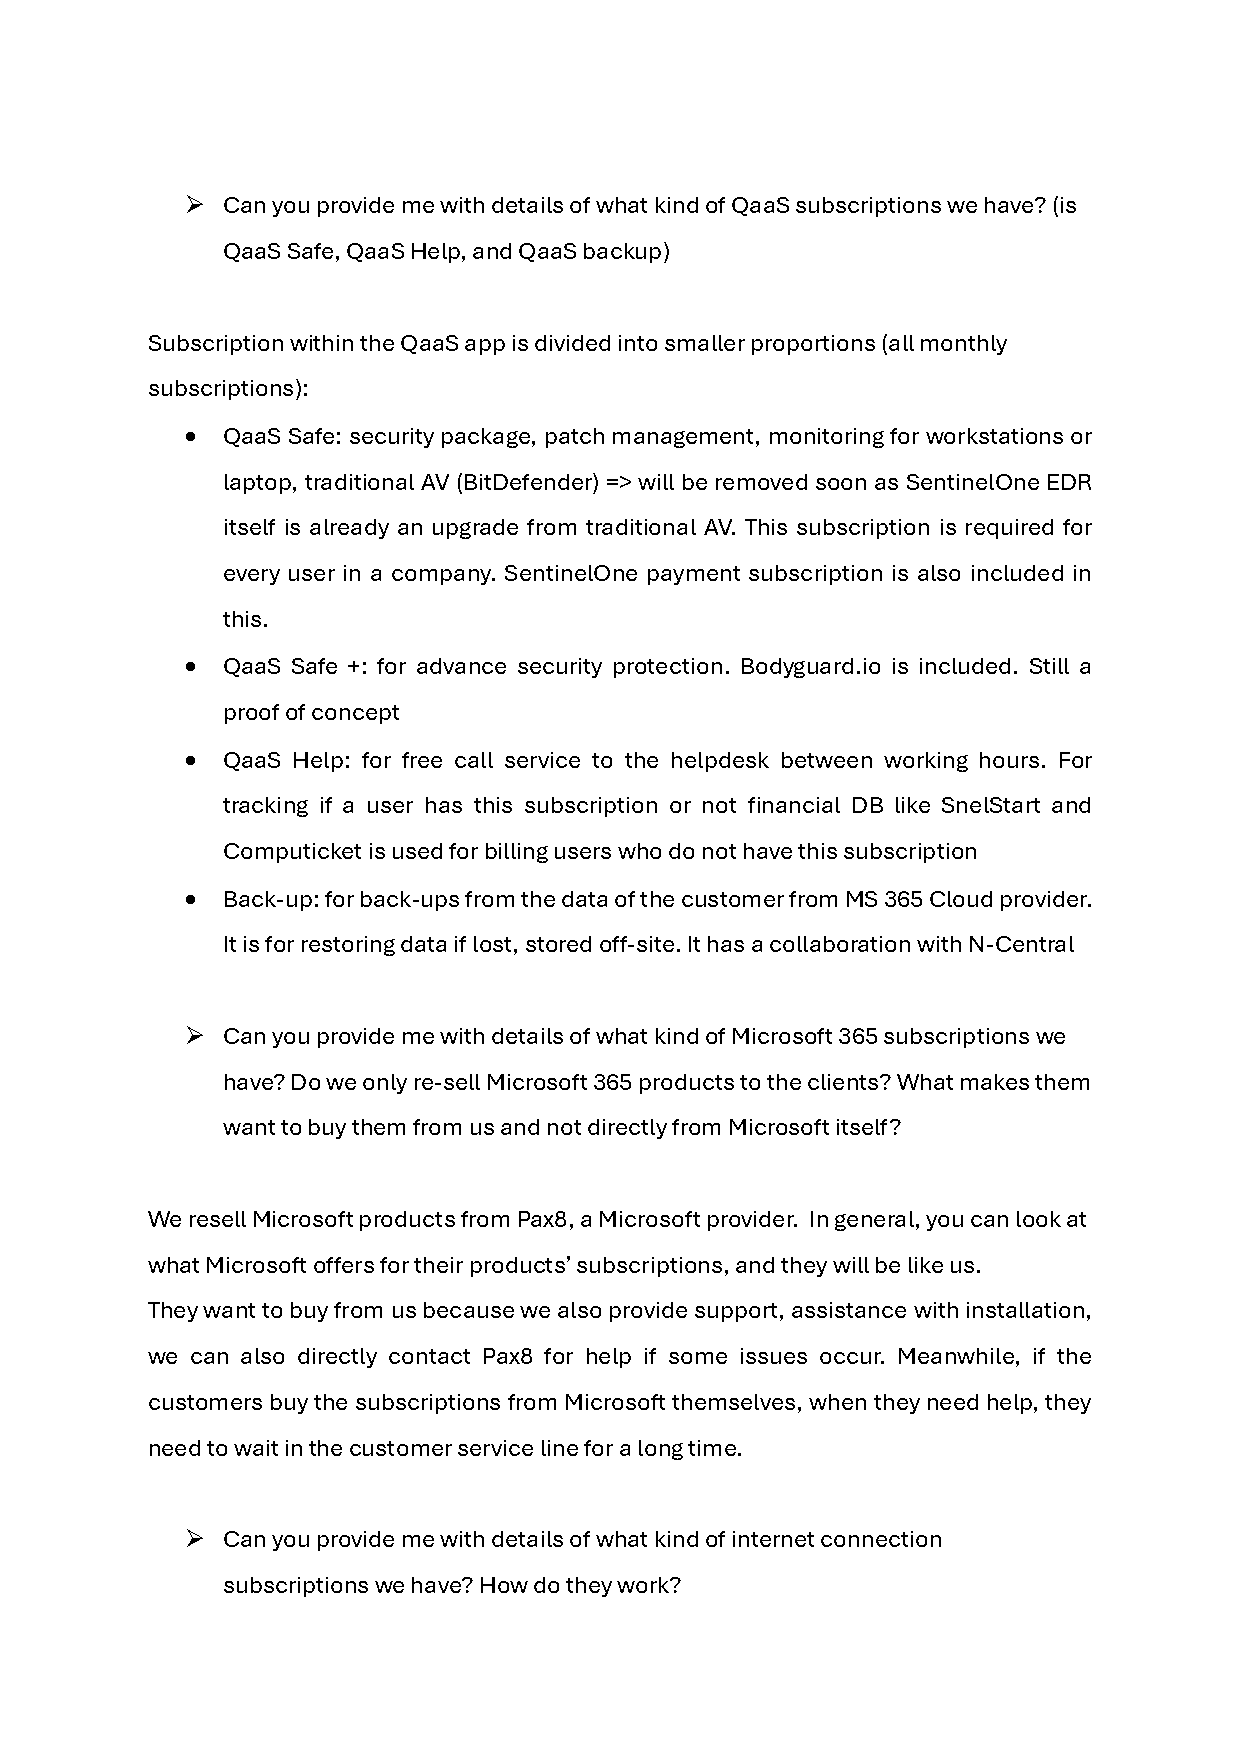
\includepdf[pages=-]{Appendices/QaaS App Subscriptions Transcript.pdf}
\newpage

\end{document}